\chapter{The Intrinsic Semiconductor}
\label{ch:intrinsic-semiconductor}

The device-oriented development in Sze and Lee begins with energy bands,
density of states, Fermi--Dirac occupation, and the equality of thermally
generated electron and hole populations \cite[Sec.~1.5]{szeLee2012}.  This
chapter follows that sequence but exposes the solid-state derivation underneath
its effective densities of states.  The full Fermi-integral formulation and
degeneracy limits are compared with Sze and Ng \cite[Sec.~1.4]{szeNg2007},
while the tensor effective-mass and state-counting steps follow the more
explicit periodic-crystal treatment developed by Rudan
\cite[Secs.~17.6.3 and 18.2--18.3]{rudan2015}.

\section{What intrinsic means}

\begin{definition}{Intrinsic semiconductor}{intrinsic-semiconductor}
An intrinsic semiconductor is a chemically pure, spatially uniform
semiconductor whose equilibrium mobile-carrier populations are generated by
the material's own electronic excitations rather than by intentionally added
donors or acceptors.  In the ideal bulk model,
\begin{equation}
  N_D^+=N_A^-=0,
  \qquad
  n=p=n_i.
  \label{eq:intrinsic-definition}
\end{equation}
\end{definition}

Intrinsic does not mean that the conduction band is always empty.  At
$T=0$ in the independent-particle ground-state picture, the valence band is
full and the conduction band is empty.  At finite temperature, some electrons
occupy conduction-band states.  Each such excitation leaves one unoccupied
state in the valence band, which is described as a hole.  Pair creation
therefore preserves
\begin{equation}
  N_{\text{conduction electrons}}
  =N_{\text{valence holes}},
  \label{eq:intrinsic-pair-counting}
\end{equation}
and spatial uniformity converts the equality of particle numbers into $n=p$.
The result is a counting statement and remains true even when the conduction
and valence densities of states have different shapes.

Real nominally undoped samples can contain residual impurities, native defects,
surface charge, or nonuniform electrostatic potentials.  The intrinsic model is
the reference obtained when these effects are neglected.  It is a model limit,
not a guarantee supplied by the word ``pure'' on a material label.

\section{Why a solid has bands rather than isolated levels}

An isolated atom has discrete one-electron energy levels.  When many atoms are
brought together to form a crystal, their orbitals overlap.  The electrostatic
potential experienced by an electron is no longer the potential of one isolated
atom, and the Pauli exclusion principle prevents all electrons from occupying
one identical state.  Each atomic level therefore splits into many closely
spaced crystal levels.  For a macroscopic number of unit cells, the spacing is
so small that the allowed levels are described as energy bands.

\begin{figure}[H]
  \centering
  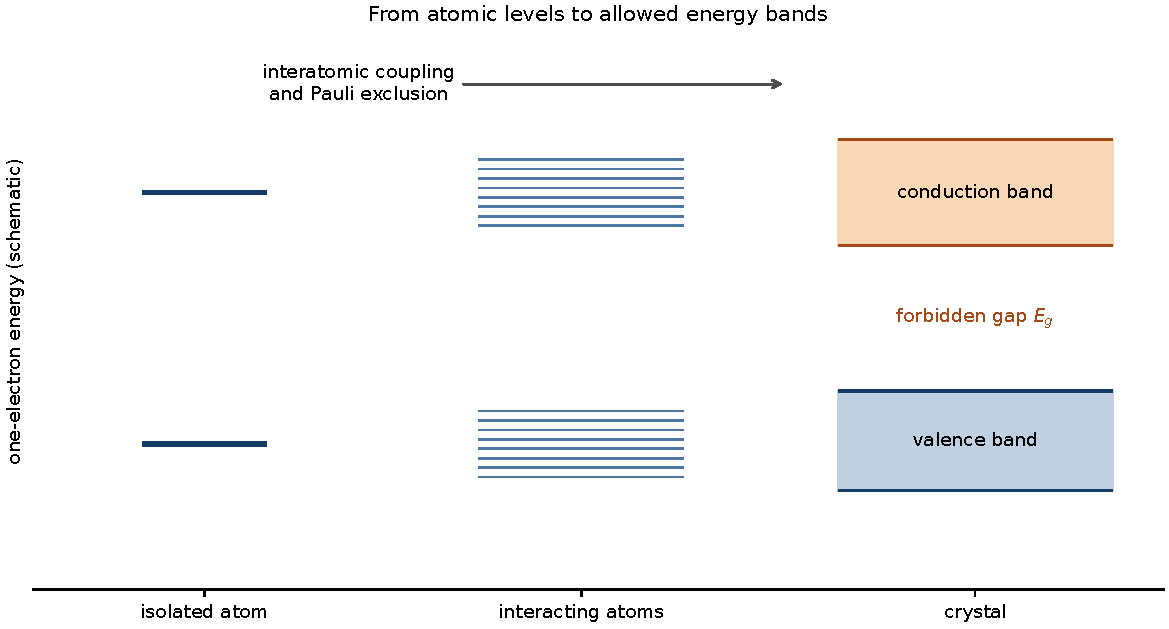
\includegraphics[width=0.78\textwidth]
    {figures/intrinsic-band-formation.pdf}
  \caption{Schematic evolution from discrete atomic levels to crystal bands.
  The drawing is a model of level splitting, not a calculated band structure.
  The number, width, and ordering of real bands must come from the crystal
  Hamiltonian.\figurenotebookmark}
  \label{fig:intrinsic-band-formation}
\end{figure}
\figurenotebooktext{figures/06_intrinsic-semiconductor/fig_06_01.ipynb}

In a covalent semiconductor such as silicon, the occupied bonding combinations
form the upper valence bands and the unoccupied antibonding combinations form
the lower conduction bands.  The energy interval between them contains no
allowed bulk eigenstates and is the forbidden gap.  This bonding picture builds
intuition, but quantitative carrier statistics require the dispersions
$E_n(\bm k)$ rather than only two horizontal band edges.

\subsection{Why neither an empty nor a full band conducts}

The semiclassical group velocity of a Bloch state is
\begin{equation}
  \bm v_n(\bm k)
  =\frac{1}{\hbar}\nabla_{\bm k}E_n(\bm k).
  \label{eq:bloch-group-velocity}
\end{equation}
In a nonmagnetic crystal with time-reversal symmetry,
\begin{equation}
  E_n(\bm k)=E_n(-\bm k),
  \qquad
  \bm v_n(-\bm k)=-\bm v_n(\bm k).
  \label{eq:time-reversal-band-velocity}
\end{equation}
An empty band carries no electronic current because it contains no electrons.
A full band also carries no net current: every occupied state at $\bm k$ has an
occupied partner at $-\bm k$ with the opposite velocity.  Written as a state
sum,
\begin{equation}
  \bm j_n
  =-\frac{q}{V}\sum_{\bm k\,\text{occupied}}\bm v_n(\bm k)
  =\bm 0
  \qquad\text{for a full band}.
  \label{eq:full-band-zero-current}
\end{equation}
Here $q>0$ is the magnitude of the electron charge.  Conductivity requires a
band to be only partially occupied so that an applied field can create an
imbalance between opposite velocities.

\subsection{Why an empty valence state is called a hole}

Suppose a valence band is full except for a small collection of empty states.
Because the velocity sum over the full band vanishes,
\begin{equation}
\begin{aligned}
  \sum_{\mathrm{occupied}}\bm v_v
  &=\sum_{\mathrm{full\ band}}\bm v_v
    -\sum_{\mathrm{empty}}\bm v_v\\
  &=-\sum_{\mathrm{empty}}\bm v_v.
\end{aligned}
  \label{eq:occupied-empty-velocity-sum}
\end{equation}
The electronic current of the almost-full band is consequently
\begin{equation}
  \bm j_v
  =-\frac{q}{V}\sum_{\mathrm{occupied}}\bm v_v
  =+\frac{q}{V}\sum_{\mathrm{empty}}\bm v_v.
  \label{eq:hole-current-equivalence}
\end{equation}
Thus the missing electronic states can be represented by positively charged
quasiparticles: holes.  The hole description is not the claim that a positively
charged fundamental particle has appeared inside the atom.  It is an exact and
convenient rewriting of the dynamics of a nearly full band.

When thermal energy promotes one valence electron into the conduction band, the
result is simultaneously one conduction electron and one valence hole.  This
solid-state picture is the origin of intrinsic pair generation and, in a
uniform ideal crystal, the equality $n=p$.

\section{From a periodic solid to band edges}

For a perfect crystal, lattice translation symmetry allows one-electron states
to be labeled by a band index $n$ and crystal wave vector $\bm k$.  Solving the
Bloch Hamiltonian gives the band functions
\begin{equation}
  H(\bm k)\ket{u_{n\bm k}}
  =E_n(\bm k)\ket{u_{n\bm k}}.
  \label{eq:bloch-band-eigenproblem}
\end{equation}
The highest occupied band at $T=0$ is called the valence band, and the next
available band is called the conduction band.  Their relevant extrema are
\begin{align}
  \Ec&=\min_{\bm k}E_c(\bm k),
  \label{eq:conduction-band-minimum}\\
  \Ev&=\max_{\bm k}E_v(\bm k),
  \label{eq:valence-band-maximum}\\
  \Eg&=\Ec-\Ev.
  \label{eq:intrinsic-band-gap}
\end{align}
If the extrema occur at the same crystal wave vector, the fundamental gap is
direct; otherwise it is indirect.  This distinction is essential for optical
and recombination processes.  For equilibrium carrier counting, the immediate
requirements are the edge energies, the number of equivalent extrema, and the
local shape of each band.

\subsection{Quadratic expansion at a conduction minimum}

Let $\bm k_c^{(a)}$ denote conduction minimum $a$, and define
$\bm q=\bm k-\bm k_c^{(a)}$.  Taylor expansion gives
\begin{equation}
\begin{aligned}
  E_c(\bm k_c^{(a)}+\bm q)
  ={}&\Ec
  +\left.\nabla_{\bm k}E_c\right|_{\bm k_c^{(a)}}\!\cdot\bm q\\
  &+\frac12\bm q^{\mathsf T}
    \left.\nabla_{\bm k}\nabla_{\bm k}E_c\right|_{\bm k_c^{(a)}}
    \bm q
  +\mathcal O(q^3).
\end{aligned}
  \label{eq:conduction-taylor-expansion}
\end{equation}
The gradient vanishes at the extremum.  Define the inverse effective-mass
tensor by
\begin{equation}
  \left(\bm M_{c,a}^{*-1}\right)_{ij}
  =\frac{1}{\hbar^2}
    \left.
    \frac{\partial^2E_c}{\partial k_i\partial k_j}
    \right|_{\bm k_c^{(a)}}.
  \label{eq:conduction-inverse-effective-mass}
\end{equation}
Then the local dispersion is
\begin{equation}
  E_c(\bm k_c^{(a)}+\bm q)
  \simeq
  \Ec+\frac{\hbar^2}{2}
  \bm q^{\mathsf T}\bm M_{c,a}^{*-1}\bm q.
  \label{eq:conduction-parabolic-band}
\end{equation}
At a genuine minimum, the Hessian and the mass tensor are positive definite.
In their principal-axis frame,
\begin{equation}
  E_c-\Ec
  =\frac{\hbar^2}{2}
  \left(
    \frac{q_1^2}{m_{c1}}
   +\frac{q_2^2}{m_{c2}}
   +\frac{q_3^2}{m_{c3}}
  \right).
  \label{eq:conduction-principal-masses}
\end{equation}

\subsection{Valence maxima and positive hole masses}

At a valence maximum the electronic Hessian is negative definite.  It is useful
to measure the missing-electron energy downward from $\Ev$ and define a
positive hole-mass tensor:
\begin{equation}
  \Ev-E_v(\bm k_v^{(b)}+\bm q)
  \simeq
  \frac{\hbar^2}{2}
  \bm q^{\mathsf T}\bm M_{v,b}^{*-1}\bm q.
  \label{eq:valence-parabolic-band}
\end{equation}
The sign change does not alter the electronic band.  It changes the description
from electrons near a maximum with negative curvature to holes with positive
excitation energy and positive effective mass.

\begin{boundarybox}
The effective-mass approximation is local.  It preserves the band-edge energy
and quadratic curvature, but it discards nonparabolicity, warping, remote
valleys, and finite bandwidth.  A carrier integral that samples far from the
edge can invalidate the approximation even when the algebra is exact.
\end{boundarybox}

\section{Applying state counting to intrinsic band edges}

\Cref{ch:band-to-density-of-states} derived the density of states from discrete
level multiplicity and the reciprocal-space count of a general band.  We now
apply that construction specifically to the ellipsoidal conduction and valence
band edges of an intrinsic bulk semiconductor.  The repeated intermediate
steps make every mass and degeneracy factor visible in this first material
application.

Begin in one dimension with a cell of length $L_x$.  Periodicity requires a
plane-wave factor to reproduce itself after translation by the cell length:
\begin{equation}
  e^{ik_x(x+L_x)}=e^{ik_xx}.
  \label{eq:periodic-plane-wave-condition}
\end{equation}
After cancelling $e^{ik_xx}$,
\begin{equation}
  e^{ik_xL_x}=1
  \quad\Longrightarrow\quad
  k_xL_x=2\pi n_x,
  \qquad n_x\in\mathbb Z.
  \label{eq:one-dimensional-k-quantization}
\end{equation}
Thus
\begin{equation}
  k_{x,n}=\frac{2\pi n_x}{L_x},
  \qquad
  \Delta k_x=k_{x,n}-k_{x,n-1}=\frac{2\pi}{L_x}.
  \label{eq:one-dimensional-k-spacing}
\end{equation}

Now place the crystal in a periodic rectangular cell of volume
$V=L_xL_yL_z$.  Applying the same argument independently along each axis gives
\begin{equation}
  k_i=\frac{2\pi n_i}{L_i},
  \qquad n_i\in\mathbb Z,
  \qquad i\in\{x,y,z\}.
  \label{eq:periodic-three-dimensional-wave-vectors}
\end{equation}
Each allowed $\bm k$ point therefore occupies reciprocal-space volume
\begin{equation}
  \Delta^3k
  =\frac{(2\pi)^3}{V}.
  \label{eq:k-space-cell-volume}
\end{equation}
The reciprocal-space point density is the inverse of this cell volume:
\begin{equation}
  \frac{1}{\Delta^3k}
  =\frac{V}{(2\pi)^3}.
  \label{eq:k-space-point-density}
\end{equation}
Including spin degeneracy $g_s$, the number of one-particle states in a small
reciprocal-space volume is
\begin{equation}
  \dd N
  =g_s\frac{V}{(2\pi)^3}\,\dd^3k.
  \label{eq:k-space-state-counting}
\end{equation}
The finite cell gives a discrete lattice of wave vectors.  The thermodynamic
limit sends each $L_i\to\infty$, so each $\Delta k_i\to0$ and the discrete sum
becomes a continuum integral.  The factor $V/(2\pi)^3$ survives this limit and
is the origin of the volume normalization in the density of states.

\subsection{The conduction-band ellipsoid}

For one ellipsoidal valley, let
\begin{equation}
  \varepsilon=E-\Ec\ge0.
  \label{eq:conduction-edge-energy}
\end{equation}
The surface of constant $\varepsilon$ in
\cref{eq:conduction-principal-masses} has semiaxes
\begin{equation}
  q_i^{\max}
  =\frac{\sqrt{2m_{ci}\varepsilon}}{\hbar}.
  \label{eq:constant-energy-ellipsoid-axes}
\end{equation}
Its enclosed reciprocal-space volume is
\begin{equation}
\begin{aligned}
  \Omega_k(\varepsilon)
  &=\frac{4\pi}{3}
    \prod_{i=1}^{3}q_i^{\max}\\
  &=\frac{4\pi}{3}
    \left(\frac{2\varepsilon}{\hbar^2}\right)^{3/2}
    \sqrt{m_{c1}m_{c2}m_{c3}}.
\end{aligned}
  \label{eq:ellipsoid-k-volume}
\end{equation}
Define the per-valley density-of-states mass
\begin{equation}
  m_{c,d}
  =\left(m_{c1}m_{c2}m_{c3}\right)^{1/3}.
  \label{eq:conduction-dos-mass}
\end{equation}
Then $\sqrt{m_{c1}m_{c2}m_{c3}}=m_{c,d}^{3/2}$.
For $g_{v,c}$ equivalent valleys, the number of states per volume with energy
between $\Ec$ and $\Ec+\varepsilon$ is
\begin{equation}
  \frac{\mathcal N_c(\varepsilon)}{V}
  =\frac{g_sg_{v,c}}{6\pi^2}
   \left(\frac{2m_{c,d}}{\hbar^2}\right)^{3/2}
   \varepsilon^{3/2}.
  \label{eq:integrated-conduction-state-count}
\end{equation}
The integrated count scales as $\varepsilon^{3/2}$ because it counts the
volume of a three-dimensional ellipsoid.  The density of states is the number
added per energy interval.  Since $\varepsilon=E-\Ec$,
\begin{equation}
\begin{aligned}
  g_c(E)
  &=\frac{1}{V}\frac{\dd\mathcal N_c}{\dd E}\\
  &=\frac{g_sg_{v,c}}{6\pi^2}
    \left(\frac{2m_{c,d}}{\hbar^2}\right)^{3/2}
    \frac{\dd}{\dd E}(E-\Ec)^{3/2}\\
  &=\frac{g_sg_{v,c}}{4\pi^2}
    \left(\frac{2m_{c,d}}{\hbar^2}\right)^{3/2}
    \sqrt{E-\Ec}.
\end{aligned}
  \label{eq:conduction-dos-differentiation}
\end{equation}
Including the fact that no conduction states occur below $\Ec$ gives
\begin{equation}
  \boxed{
  g_c(E)
  =\frac{g_sg_{v,c}}{4\pi^2}
   \left(\frac{2m_{c,d}}{\hbar^2}\right)^{3/2}
   \sqrt{E-\Ec}\,\Theta(E-\Ec).
  }
  \label{eq:conduction-density-of-states}
\end{equation}

\begin{figure}[H]
  \centering
  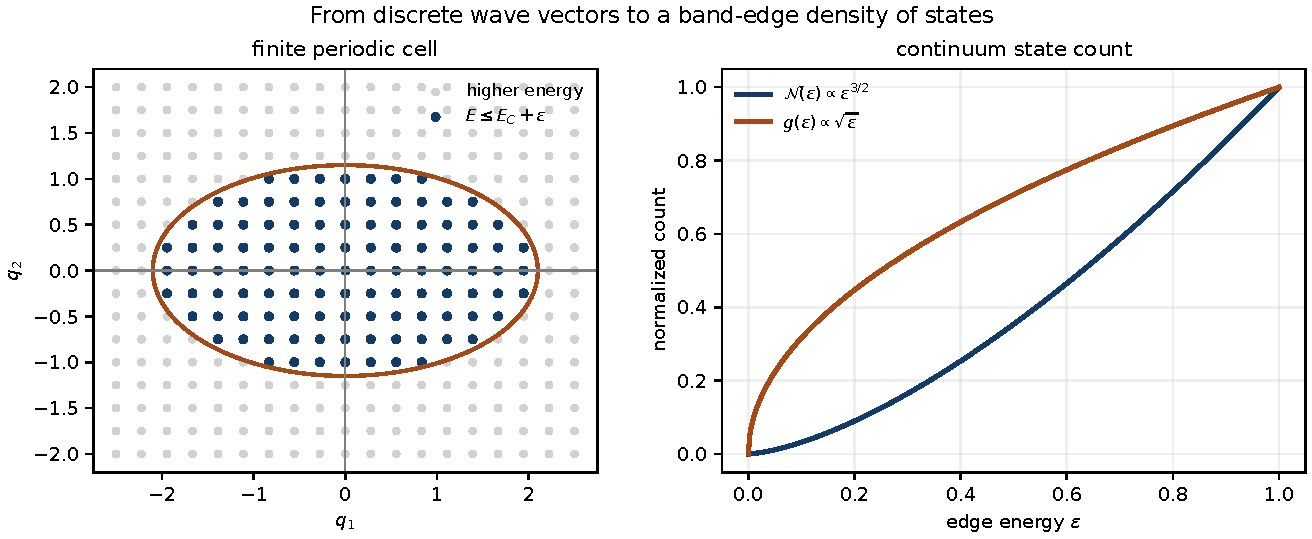
\includegraphics[width=0.90\textwidth]
    {figures/intrinsic-kspace-state-counting.pdf}
  \caption{A finite periodic cell supplies discrete wave vectors.  Counting
  points inside the constant-energy ellipsoid gives an integrated count
  proportional to $\varepsilon^{3/2}$; differentiation produces the familiar
  three-dimensional square-root density of states.  Only a two-dimensional
  cross-section of the ellipsoid is drawn.\figurenotebookmark}
  \label{fig:intrinsic-kspace-state-counting}
\end{figure}
\figurenotebooktext{figures/06_intrinsic-semiconductor/fig_06_02.ipynb}
The factor $g_s$ counts spin, $g_{v,c}$ counts equivalent valleys, and
$m_{c,d}$ accounts for the shape of each valley.  A quoted effective mass that
already absorbs valley degeneracy must not be multiplied by $g_{v,c}$ again.

\subsection{The valence-band density of states}

The same counting argument, now using the positive hole energy
$\varepsilon_h=\Ev-E$, gives
\begin{equation}
  \boxed{
  g_v(E)
  =\frac{g_sg_{v,v}}{4\pi^2}
   \left(\frac{2m_{v,d}}{\hbar^2}\right)^{3/2}
   \sqrt{\Ev-E}\,\Theta(\Ev-E).
  }
  \label{eq:valence-density-of-states}
\end{equation}
If several inequivalent valleys or valence bands contribute, their densities of
states must be summed:
\begin{equation}
  g_c(E)=\sum_a g_{c,a}(E),
  \qquad
  g_v(E)=\sum_b g_{v,b}(E).
  \label{eq:multiband-dos-sum}
\end{equation}
For degenerate isotropic heavy- and light-hole bands with a common maximum,
this sum can be represented by
\begin{equation}
  m_{v,d}
  =\left(m_{hh}^{3/2}+m_{lh}^{3/2}\right)^{2/3},
  \label{eq:combined-hole-dos-mass}
\end{equation}
provided spin and band degeneracies are handled consistently.

\section{Combining available states with statistical occupation}

The density of states answers, ``How many states are available?''  It contains
no temperature and no chemical potential.  The partition-function derivation
in \cref{ch:statistical-mechanics-carriers} answers the independent question,
``With what probability is each state occupied?''  We briefly restate the
single-state result before applying it to the intrinsic bands.

\subsection{One-state partition-function recap}

A one-electron state of energy $E$ can contain either zero or one electron of a
given spin label.  In equilibrium with a particle and energy reservoir, its two
grand-canonical weights are
\begin{equation}
  w_0=1,
  \qquad
  w_1=e^{-\beta(E-\mu)},
  \qquad
  \beta=\frac{1}{\kb T}.
  \label{eq:single-fermion-state-weights}
\end{equation}
The single-state grand partition function is the sum
\begin{equation}
  \mathcal Z_E=w_0+w_1
  =1+e^{-\beta(E-\mu)}.
  \label{eq:single-fermion-grand-partition}
\end{equation}
The mean occupation is the occupied value, one, times its normalized
probability:
\begin{equation}
\begin{aligned}
  f(E,\mu,T)
  &=\frac{1\times w_1+0\times w_0}{\mathcal Z_E}\\
  &=\frac{e^{-\beta(E-\mu)}}
          {1+e^{-\beta(E-\mu)}}\\
  &=\frac{1}{1+e^{(E-\mu)/(\kb T)}}.
\end{aligned}
  \label{eq:fermi-dirac-from-single-state-partition}
\end{equation}
Pauli exclusion is what restricts the occupation to zero or one and produces
the plus sign in the denominator.

An electronic state is empty with probability
\begin{equation}
\begin{aligned}
  1-f(E,\mu,T)
  &=1-\frac{1}{1+e^{(E-\mu)/(\kb T)}}\\
  &=\frac{1}{1+e^{(\mu-E)/(\kb T)}}.
\end{aligned}
  \label{eq:empty-state-probability}
\end{equation}
This is the probability used to count holes in a valence band.

\subsection{Spectral carrier densities}

The Fermi--Dirac function answers, ``What is the probability that each
electronic state is occupied?''  The carrier spectral densities are the
products of state availability and the relevant probability:
\begin{align}
  \mathcal n(E)&=g_c(E)f(E,\mu,T),
  \label{eq:electron-spectral-density}\\
  \mathcal p(E)&=g_v(E)\bigl[1-f(E,\mu,T)\bigr].
  \label{eq:hole-spectral-density}
\end{align}
Their areas are the carrier concentrations.

\begin{figure}[H]
  \centering
  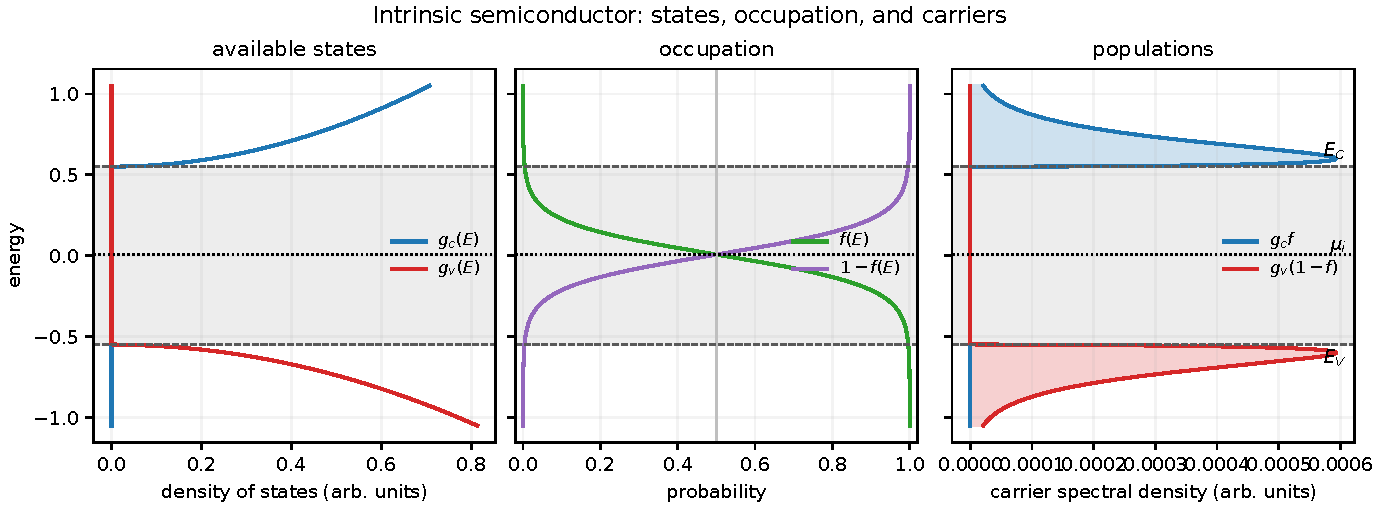
\includegraphics[width=0.96\textwidth]
    {figures/intrinsic-states-occupation.pdf}
  \caption{Available states, occupation probabilities, and carrier spectral
  densities are distinct quantities.  The gray interval is the forbidden gap,
  where the density of states is zero.  The unequal model prefactors illustrate
  that intrinsic neutrality requires equal areas, not mirror-symmetric curves.\figurenotebookmark}
  \label{fig:intrinsic-states-occupation}
\end{figure}
\figurenotebooktext{figures/06_intrinsic-semiconductor/fig_06_03.ipynb}

\section{Exact parabolic-band carrier integrals}

Start with the electron concentration
\begin{equation}
  n
  =\int_{\Ec}^{\infty}
    \frac{g_c(E)}{1+\exp[(E-\mu)/(\kb T)]}\,\dd E.
  \label{eq:exact-electron-integral}
\end{equation}
Introduce
\begin{equation}
  x=\frac{E-\Ec}{\kb T},
  \qquad
  \eta_c=\frac{\mu-\Ec}{\kb T}.
  \label{eq:electron-fermi-integral-variables}
\end{equation}
Then $E-\Ec=x\kb T$ and $\dd E=\kb T\,\dd x$.  Substitution gives
\begin{equation}
\begin{aligned}
  n
  ={}&\frac{g_sg_{v,c}}{4\pi^2}
      \left(\frac{2m_{c,d}}{\hbar^2}\right)^{3/2}
      (\kb T)^{3/2}\\
     &\times
      \int_0^\infty
      \frac{\sqrt{x}}{1+e^{x-\eta_c}}\,\dd x.
\end{aligned}
  \label{eq:electron-integral-dimensionless}
\end{equation}
Define the normalized Fermi--Dirac integral
\begin{equation}
  F_{1/2}(\eta)
  =\frac{2}{\sqrt\pi}
   \int_0^\infty
   \frac{\sqrt{x}}{1+e^{x-\eta}}\,\dd x.
  \label{eq:normalized-fermi-integral-half}
\end{equation}
Different books normalize Fermi integrals differently; the prefactor in
\cref{eq:normalized-fermi-integral-half} is part of our definition.  With this
convention,
\begin{equation}
  \boxed{
  n=\Nc F_{1/2}(\eta_c),
  \qquad
  \Nc=g_sg_{v,c}
  \left(\frac{m_{c,d}\kb T}{2\pi\hbar^2}\right)^{3/2}.
  }
  \label{eq:exact-electron-concentration-fermi-integral}
\end{equation}
For $g_s=2$, the effective density of states can also be written
\begin{equation}
  \Nc
  =2g_{v,c}
   \left(\frac{2\pi m_{c,d}\kb T}{h^2}\right)^{3/2}.
  \label{eq:conduction-effective-density-h}
\end{equation}
Introduce the thermal de Broglie wavelength associated with the conduction DOS
mass,
\begin{equation}
  \lambda_{T,c}
  =\frac{h}{\sqrt{2\pi m_{c,d}\kb T}}.
  \label{eq:conduction-thermal-wavelength}
\end{equation}
Then
\begin{equation}
  \Nc=\frac{g_sg_{v,c}}{\lambda_{T,c}^3}.
  \label{eq:effective-density-thermal-volume}
\end{equation}
This form gives a useful interpretation: the effective density of states is the
degeneracy divided by a characteristic thermal wave-packet volume.  It also
makes the $T^{3/2}$ dependence immediate because
$\lambda_{T,c}\propto T^{-1/2}$.

For holes, introduce
\begin{equation}
  x=\frac{\Ev-E}{\kb T},
  \qquad
  \eta_v=\frac{\Ev-\mu}{\kb T}.
  \label{eq:hole-fermi-integral-variables}
\end{equation}
Using
\begin{equation}
  1-f(E,\mu,T)
  =\frac{1}{1+\exp[(\mu-E)/(\kb T)]},
  \label{eq:hole-occupation-probability}
\end{equation}
produces
\begin{equation}
  \boxed{
  p=\Nv F_{1/2}(\eta_v),
  \qquad
  \Nv=g_sg_{v,v}
  \left(\frac{m_{v,d}\kb T}{2\pi\hbar^2}\right)^{3/2}.
  }
  \label{eq:exact-hole-concentration-fermi-integral}
\end{equation}
These equations retain Fermi--Dirac statistics while still assuming local
parabolic bands.

\section{The nondegenerate limit}

An intrinsic semiconductor with $\Eg\gg\kb T$ normally has its chemical
potential several thermal energies from either band edge.  To see the
approximation directly, define
\begin{equation}
  y=\frac{E-\mu}{\kb T}>0.
  \label{eq:reduced-energy-boltzmann-tail}
\end{equation}
The exact occupation can be rewritten as
\begin{equation}
  f(E)=\frac{e^{-y}}{1+e^{-y}}.
  \label{eq:fermi-tail-rewritten}
\end{equation}
When $e^{-y}\ll1$, the denominator approaches one and
\begin{equation}
  f(E)\simeq e^{-y}
  =\exp\left[-\frac{E-\mu}{\kb T}\right].
  \label{eq:single-state-boltzmann-approximation}
\end{equation}
The relative overestimate made by replacing $f$ with $e^{-y}$ is especially
simple:
\begin{equation}
  \frac{e^{-y}-f}{f}=e^{-y}.
  \label{eq:boltzmann-relative-error}
\end{equation}
At $E-\mu=3\kb T$, it is about $e^{-3}\simeq5\%$; farther into the tail it
falls exponentially.

The same limit can be taken inside the normalized Fermi integral.  If
$\eta\ll-1$,
\begin{equation}
  \frac{1}{1+e^{x-\eta}}
  \simeq e^{\eta-x}.
  \label{eq:fermi-integral-integrand-boltzmann-limit}
\end{equation}
Therefore
\begin{equation}
\begin{aligned}
  F_{1/2}(\eta)
  &\simeq\frac{2e^\eta}{\sqrt\pi}
    \int_0^\infty x^{1/2}e^{-x}\,\dd x\\
  &=\frac{2e^\eta}{\sqrt\pi}
    \Gamma\left(\frac32\right)\\
  &=\frac{2e^\eta}{\sqrt\pi}
    \frac{\sqrt\pi}{2}\\
  &=e^\eta.
\end{aligned}
  \label{eq:fermi-integral-boltzmann-limit}
\end{equation}

\begin{figure}[H]
  \centering
  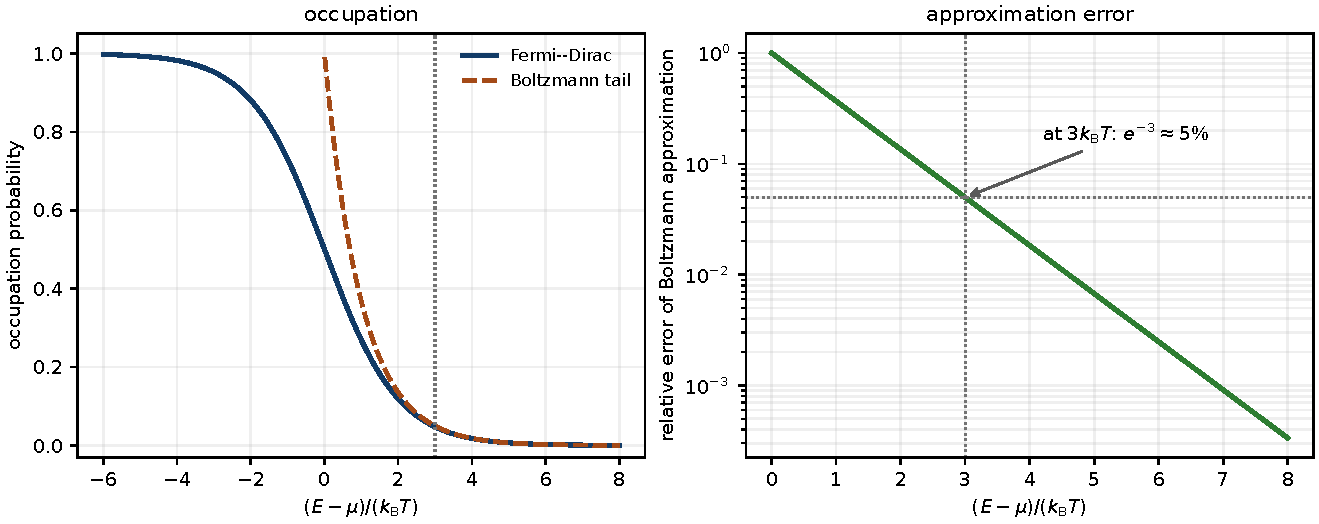
\includegraphics[width=0.88\textwidth]
    {figures/intrinsic-fermi-boltzmann.pdf}
  \caption{Exact Fermi--Dirac occupation and its Boltzmann-tail approximation.
  The right panel makes the approximation error explicit instead of treating
  ``several $\kb T$'' as an unexamined rule.\figurenotebookmark}
  \label{fig:intrinsic-fermi-boltzmann}
\end{figure}
\figurenotebooktext{figures/06_intrinsic-semiconductor/fig_06_04.ipynb}

The carrier concentrations then become
\begin{align}
  n
  &\simeq\Nc
   \exp\left[-\frac{\Ec-\mu}{\kb T}\right],
  \label{eq:nondegenerate-electron-concentration}\\
  p
  &\simeq\Nv
   \exp\left[-\frac{\mu-\Ev}{\kb T}\right].
  \label{eq:nondegenerate-hole-concentration}
\end{align}
The exponential factors describe occupation; $\Nc$ and $\Nv$ describe the
number of thermally accessible states near the edges.  They play different
roles and should not be merged conceptually.

\begin{modelcheck}
The exact and nondegenerate calculations should be compared at selected
conditions.  Agreement establishes that the Boltzmann reduction is adequate
for that case; it does not establish that every doped or high-temperature case
will remain nondegenerate.
\end{modelcheck}

\section{Deriving the intrinsic chemical potential}

Set $n=p$ in
\cref{eq:nondegenerate-electron-concentration,eq:nondegenerate-hole-concentration}:
\begin{equation}
  \Nc e^{-(\Ec-\mui)/(\kb T)}
  =\Nv e^{-(\mui-\Ev)/(\kb T)}.
  \label{eq:intrinsic-neutrality-exponentials}
\end{equation}
Taking the natural logarithm gives
\begin{equation}
  \ln\Nc-\frac{\Ec-\mui}{\kb T}
  =\ln\Nv-\frac{\mui-\Ev}{\kb T}.
  \label{eq:intrinsic-neutrality-logarithm}
\end{equation}
Collecting the two $\mui$ terms yields
\begin{equation}
  2\mui
  =\Ec+\Ev+\kb T\ln\left(\frac{\Nv}{\Nc}\right),
  \label{eq:intrinsic-chemical-potential-intermediate}
\end{equation}
and therefore
\begin{equation}
  \boxed{
  \mui
  =\frac{\Ec+\Ev}{2}
   +\frac{\kb T}{2}
    \ln\left(\frac{\Nv}{\Nc}\right).
  }
  \label{eq:intrinsic-chemical-potential}
\end{equation}
The intrinsic chemical potential equals midgap only when the effective
conduction and valence state counts are equal.  If the spin factors cancel,
substitution of the effective densities gives
\begin{equation}
  \mui-E_{\mathrm{mid}}
  =\frac{\kb T}{2}
    \ln\left(\frac{g_{v,v}}{g_{v,c}}\right)
   +\frac{3\kb T}{4}
    \ln\left(\frac{m_{v,d}}{m_{c,d}}\right),
  \label{eq:intrinsic-level-mass-degeneracy-shift}
\end{equation}
where $E_{\mathrm{mid}}=(\Ec+\Ev)/2$.  More valence-band states shift $\mui$
toward the conduction band so that their smaller empty fraction still produces
the same number of holes as electrons.  More conduction-band states produce the
opposite shift.

\section{Deriving the intrinsic carrier concentration}

Multiply the nondegenerate electron and hole concentrations:
\begin{equation}
\begin{aligned}
  np
  &=\Nc\Nv
    \exp\left[-\frac{\Ec-\mu+\mu-\Ev}{\kb T}\right]\\
  &=\Nc\Nv
    \exp\left(-\frac{\Eg}{\kb T}\right).
\end{aligned}
  \label{eq:mass-action-derivation}
\end{equation}
In an intrinsic semiconductor $n=p=n_i$, hence
\begin{equation}
  \boxed{
  n_i
  =\sqrt{\Nc\Nv}
   \exp\left(-\frac{\Eg}{2\kb T}\right).
  }
  \label{eq:intrinsic-carrier-concentration}
\end{equation}
The factor of two in the exponential denominator has a physical counting
origin: one thermal excitation creates two mobile quasiparticles, but it costs
approximately one band-gap energy to create the pair.

Equation~\eqref{eq:mass-action-derivation} also gives the equilibrium mass-action
law
\begin{equation}
  np=n_i^2.
  \label{eq:mass-action-law}
\end{equation}
This simple form uses nondegenerate statistics and a common equilibrium chemical
potential.  In a degenerate semiconductor the exact Fermi integrals must replace
the exponentials, so $np=n_i^2$ is not generally preserved in this form
\cite[Sec.~1.4.1]{szeNg2007}.

\section{Temperature dependence}

If the DOS masses and degeneracies are treated as constants,
\begin{equation}
  \Nc\propto T^{3/2},
  \qquad
  \Nv\propto T^{3/2}.
  \label{eq:effective-density-temperature-scaling}
\end{equation}
Consequently,
\begin{equation}
  n_i(T)
  \propto T^{3/2}
  \exp\left[-\frac{\Eg(T)}{2\kb T}\right].
  \label{eq:intrinsic-temperature-scaling}
\end{equation}
The gap itself usually changes with temperature.  A common interpolation is
\begin{equation}
  \Eg(T)
  =\Eg(0)-\frac{\alpha T^2}{T+\beta},
  \label{eq:varshni-gap}
\end{equation}
with material-specific parameters $\alpha$ and $\beta$.  This compact law is
useful only over the range supported by the fitted data.

Taking the logarithmic derivative of
\cref{eq:intrinsic-temperature-scaling} gives
\begin{equation}
  \frac{\dd\ln n_i}{\dd T}
  =\frac{3}{2T}
   -\frac{1}{2\kb T}\frac{\dd\Eg}{\dd T}
   +\frac{\Eg}{2\kb T^2},
  \label{eq:intrinsic-log-temperature-derivative}
\end{equation}
when mass temperature dependence is neglected.  For an ordinary semiconductor,
the last term is large and positive; a decreasing gap adds another positive
contribution.  This is why intrinsic concentration can change by many orders of
magnitude over an experimentally modest temperature interval.

If $\Eg$ is nearly constant over a restricted range,
\begin{equation}
  \ln\left(\frac{n_i}{T^{3/2}}\right)
  =\text{constant}-\frac{\Eg}{2\kb}\frac{1}{T}.
  \label{eq:intrinsic-arrhenius-linearization}
\end{equation}
A plot of $\ln(n_i/T^{3/2})$ against $1/T$ is then approximately linear with
slope $-\Eg/(2\kb)$.  Curvature can reflect $\Eg(T)$, temperature-dependent
masses, or failure of the adopted band model.

For the illustrative silicon calculation in
\cref{fig:intrinsic-temperature-dependence}, the gap interpolation parameters
follow the convention summarized by Sze and Ng \cite[Fig.~1.6]{szeNg2007}, and
the room-temperature effective densities follow Sze and Lee
\cite[Sec.~1.5]{szeLee2012}.  Their joint use is declared explicitly so that a
later edition can replace them as one parameter set rather than silently mixing
new and old values.

\begin{figure}[H]
  \centering
  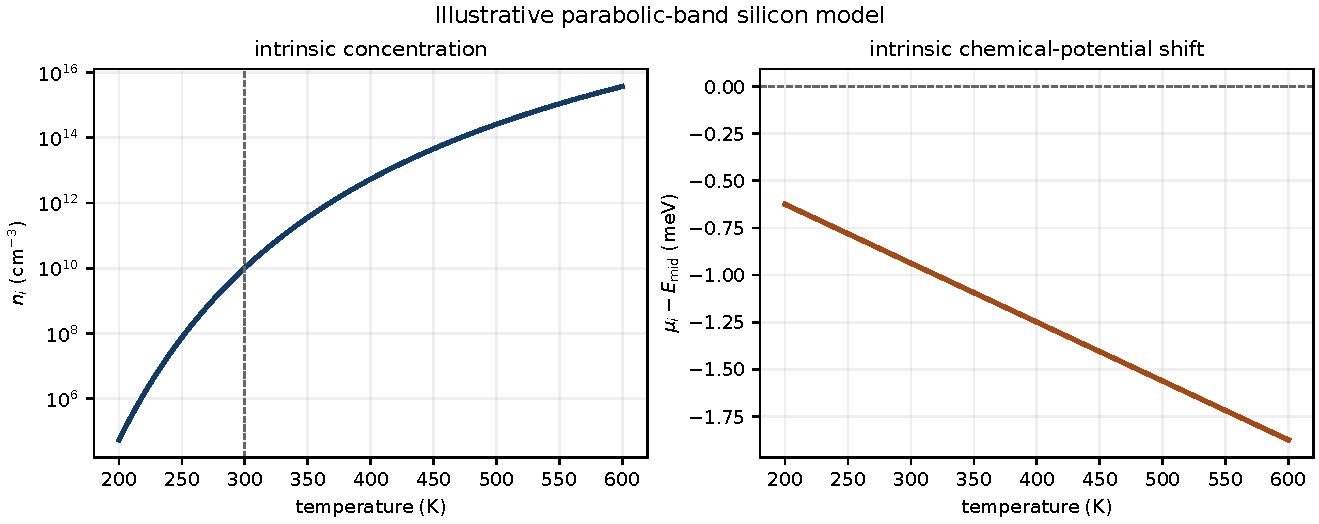
\includegraphics[width=0.90\textwidth]
    {figures/intrinsic-temperature-dependence.pdf}
  \caption{Illustrative silicon parabolic-band calculation using
  $\Eg(0)=\SI{1.169}{\electronvolt}$,
  $\alpha=\SI{4.9e-4}{\electronvolt\per\kelvin}$,
  $\beta=\SI{655}{\kelvin}$,
  $\Nc(\SI{300}{\kelvin})=\SI{2.86e19}{\per\cubic\centi\metre}$, and
  $\Nv(\SI{300}{\kelvin})=\SI{2.66e19}{\per\cubic\centi\metre}$.
  The concentration is exponentially temperature-sensitive, whereas the
  intrinsic-level displacement from midgap remains on the millielectronvolt
  scale for these parameters.  The numbers illustrate one internally
  consistent convention rather than immutable material constants.\figurenotebookmark}
  \label{fig:intrinsic-temperature-dependence}
\end{figure}
\figurenotebooktext{figures/06_intrinsic-semiconductor/fig_06_05.ipynb}

\section{Worked silicon estimate at \SI{300}{\kelvin}}

Using the same Sze--Lee effective-density convention for a transparent control
calculation \cite[Sec.~1.5]{szeLee2012}, take
\begin{equation}
\begin{aligned}
  T&=\SI{300}{\kelvin},
  &\kb T&=\SI{0.02585}{\electronvolt},\\
  \Eg&=\SI{1.12}{\electronvolt},
  &\Nc&=\SI{2.86e19}{\per\cubic\centi\metre},\\
  &&\Nv&=\SI{2.66e19}{\per\cubic\centi\metre}.
\end{aligned}
  \label{eq:silicon-example-inputs}
\end{equation}
The intrinsic-level displacement from midgap is
\begin{equation}
\begin{aligned}
  \mui-E_{\mathrm{mid}}
  &=\frac{\kb T}{2}\ln\left(\frac{\Nv}{\Nc}\right)\\
  &\simeq\SI{-0.94}{\milli\electronvolt}.
\end{aligned}
  \label{eq:silicon-intrinsic-level-example}
\end{equation}
The negative sign means that this particular DOS convention places $\mui$
slightly below midgap.  The intrinsic concentration is
\begin{equation}
\begin{aligned}
  n_i
  &=\sqrt{(2.86\times10^{19})(2.66\times10^{19})}
    \exp\left[-\frac{1.12}{2(0.02585)}\right]\\
  &\simeq\SI{1.1e10}{\per\cubic\centi\metre}.
\end{aligned}
  \label{eq:silicon-intrinsic-concentration-example}
\end{equation}
Published room-temperature values differ because the adopted gap, DOS masses,
valley conventions, and temperature are not identical.  Agreement should be
judged only after these definitions are aligned, not by silently adjusting a
constant until one preferred table is reproduced.

\section{When the full Fermi integrals are required}

The intrinsic parabolic-band problem can be solved without the Boltzmann
approximation.  Define
\begin{equation}
  \eta_c=\frac{\mui-\Ec}{\kb T},
  \qquad
  \eta_v=\frac{\Ev-\mui}{\kb T}.
  \label{eq:intrinsic-exact-reduced-potentials}
\end{equation}
Their sum is constrained by the gap:
\begin{equation}
  \eta_c+\eta_v=-\frac{\Eg}{\kb T}.
  \label{eq:intrinsic-reduced-potential-gap-constraint}
\end{equation}
Neutrality requires
\begin{equation}
  \Nc F_{1/2}(\eta_c)
  =\Nv F_{1/2}(\eta_v).
  \label{eq:intrinsic-exact-neutrality}
\end{equation}
Equations~\eqref{eq:intrinsic-reduced-potential-gap-constraint} and
\eqref{eq:intrinsic-exact-neutrality} determine $\mui$ without assuming
$F_{1/2}(\eta)\simeq e^\eta$.  Ordinary intrinsic Si and GaAs near room
temperature are strongly nondegenerate because $\Eg/\kb T$ is large, but the
exact form is the appropriate reference for narrow-gap materials, sufficiently
high temperatures, or numerical validation.

\section{Assumptions exposed}

The compact intrinsic formula
\cref{eq:intrinsic-carrier-concentration} depends on the following assumptions:
\begin{enumerate}
  \item the material is spatially uniform and in thermal equilibrium;
  \item donor, acceptor, and charged-defect contributions are absent;
  \item band edges are represented by quadratic dispersions;
  \item all relevant valleys and valence bands are counted consistently;
  \item the chemical potential lies far enough from the bands for
        nondegenerate statistics;
  \item the reported gap and DOS parameters refer to the same material phase
        and temperature convention; and
  \item many-body effects such as band-gap narrowing are negligible.
\end{enumerate}
Removing one assumption does not merely change a prefactor.  It can change the
neutrality equation, the required statistics, or even the meaning of the band
edges.

\section{Verification checklist}

A trustworthy intrinsic-semiconductor calculation should demonstrate that
\begin{enumerate}
  \item the DOS integrates to units of concentration;
  \item $n(\mu,T)$ increases and $p(\mu,T)$ decreases monotonically with $\mu$;
  \item the solved intrinsic state satisfies $n-p=0$ to a declared tolerance;
  \item a rigid shift of $\Ec$, $\Ev$, and $\mu$ leaves $n$ and $p$ unchanged;
  \item the full Fermi-integral result approaches the Boltzmann result in the
        nondegenerate limit;
  \item constant-mass effective densities scale as $T^{3/2}$; and
  \item the silicon control case is compared with a source using compatible
        gap and DOS conventions.
\end{enumerate}

\section{Chapter summary}

The intrinsic concentration is the endpoint of a solid-state derivation.  Band
curvature defines effective-mass tensors; periodic-boundary state counting turns
the resulting ellipsoids into square-root densities of states; Fermi--Dirac
statistics converts available states into occupied conduction states and empty
valence states; and intrinsic neutrality selects the chemical potential.  Only
then does the familiar expression
\begin{equation*}
  n_i=\sqrt{\Nc\Nv}\,e^{-\Eg/(2\kb T)}
\end{equation*}
appear.  Its compactness should not hide the chain of assumptions that makes it
valid.
